\chapter{Diseño}
\label{cap:capitulo5}

\begin{flushright}
\begin{minipage}[]{10cm}
\emph{El diseño no es solo cómo se ve o cómo se siente, sino cómo funciona.}\\
\end{minipage}\\

Steve Jobs, \textit{Apple Inc.}\\
\end{flushright}

\vspace{1cm}

En este capítulo se describe el diseño e implementación del sistema desarrollado, presentando su arquitectura general y los distintos módulos software y hardware que lo componen, así como las principales decisiones de diseño adoptadas para garantizar su correcta integración, uso y fiabilidad.\\

\section{Descripción del sistema}
\label{sec:descripcion_sistema}

El sistema propuesto consiste en un pastillero inteligente diseñado para facilitar la gestión de la medicación mediante la automatización de recordatorios y la dispensación controlada de dosis de medicamentos. Este dispositivo integra diferentes componentes electrónicos, mecánicos y módulos software que trabajan de forma conjunta para ofrecer una solución funcional, accesible y de bajo coste.\\

El sistema se estructura en diferentes módulos funcionales que trabajan de forma coordinada. Entre ellos se encuentran la unidad de control, el sistema de actuación, la interfaz de usuario, el sistema de sensado y el sistema de comunicación. En la Figura~\ref{fig:arquitectura_sistema} se muestra la arquitectura general del sistema, donde se representan los principales bloques funcionales y sus interconexiones.


\begin{figure}[H]
    \centering
    
\includegraphics[width=\textwidth]{figs/arquitectura_sistema.png}
    \caption{Arquitectura general del sistema desarrollado}
    \label{fig:arquitectura_sistema}
\end{figure}




\subsection{Módulos del sistema}

El sistema se estructura en diferentes módulos funcionales que trabajan de forma coordinada para garantizar el correcto funcionamiento del dispositivo.

\begin{itemize}

    \item \textbf{Módulo de control:} basado en un microcontrolador ESP32 (ESP32-WROOM-32), constituye el núcleo del sistema. Se encarga de la ejecución del programa principal, la gestión del tiempo, la coordinación de los distintos módulos y la toma de decisiones en función de los eventos del sistema, como la activación de una toma programada o la interacción del usuario.

    \item \textbf{Módulo de interfaz:} permite la interacción con el usuario y está compuesto por una pantalla táctil integrada y una aplicación móvil. Ambas interfaces ofrecen funcionalidades equivalentes, permitiendo configurar las tomas de medicación, consultar las tomas programadas para el día, activar el sensor biomédico y visualizar el historial de medidas registradas. Este módulo actúa como punto de entrada de información al sistema.

    \item \textbf{Módulo de actuación:} encargado de la dispensación física de la medicación. A partir de las órdenes generadas por el módulo de control, acciona los servomotores que, mediante un mecanismo basado en una rueda de Ginebra, posicionan el compartimento correspondiente para liberar la dosis en el momento adecuado.

    \item \textbf{Módulo de sensado:} compuesto por el sensor biomédico MAX30102, se encarga de la adquisición de parámetros fisiológicos del usuario, como la frecuencia cardíaca y la saturación de oxígeno en sangre. Los datos obtenidos son procesados por el módulo de control y pueden ser visualizados a través de las interfaces del sistema.

    \item \textbf{Módulo de comunicación:} permite la conexión entre el dispositivo y la aplicación móvil mediante WiFi. Este módulo gestiona tanto la configuración inicial del dispositivo como el intercambio de información durante su funcionamiento, incluyendo la sincronización de datos y el envío de credenciales de red.

\end{itemize}

\subsection{Comunicación entre módulos}

El funcionamiento del sistema se basa en la comunicación coordinada entre los distintos módulos funcionales, que intercambian información a través de diferentes interfaces y protocolos en función de su naturaleza.\\

\begin{figure}[H]
    \centering
    
\includegraphics[width=\textwidth]{figs/mod_coms_diagram.png}
    \caption{Diagrama de comunicación entre los módulos del sistema (imagen generada por IA)}
    \label{fig:comunicacion_modulos}
\end{figure}

En la Figura~\ref{fig:comunicacion_modulos} se muestra un diagrama de bloques que representa las principales interacciones entre los módulos del sistema.

El módulo de control actúa como elemento central, gestionando la comunicación con el resto de módulos. En primer lugar, se comunica con el módulo de sensado mediante el protocolo I2C, a través del cual se obtienen las mediciones del sensor biomédico. Estas lecturas son procesadas y utilizadas por el sistema para su visualización y almacenamiento.\\

Por otro lado, el módulo de control se encarga de gobernar el módulo de actuación mediante señales PWM, que permiten el control preciso de los servomotores responsables del movimiento del mecanismo que dispensa los medicamentos.\\

Respecto a la interacción con el usuario, el módulo de control se comunica con la interfaz local por medio de la pantalla táctil que lleva incorporada la ESP32-2432S08, gestionando los eventos de entrada y actualiza los datos mostrados. Además, la comunicación con la aplicación móvil se lleva a cabo mediante conexión WiFi sin hilos, lo que posibilita no solo la puesta en marcha inicial del dispositivo, sino también la sincronización de datos mientras se está usando.

\subsection{Consideraciones de diseño}
\label{sec:consideraciones_diseno}

Durante el desarrollo del sistema se han tenido en cuenta diversos criterios de diseño con el objetivo de garantizar su funcionalidad, accesibilidad y fiabilidad en un entorno doméstico.\\

En primer lugar, se ha priorizado el \textbf{bajo coste} del dispositivo, seleccionando componentes electrónicos asequibles y de fácil disponibilidad, sin comprometer las prestaciones necesarias para el correcto funcionamiento del sistema. Todos los componentes usado son adquiribles en páginas como Aliexpress donde los costes de cada componente han sido inferiores a 5\euro, de este modo el coste total del dispositivo no supera los 30\euro.\\

Asimismo, se ha prestado especial atención a la \textbf{facilidad de uso}, diseñando una interfaz sencilla e intuitiva tanto en el dispositivo como en la aplicación móvil. Para ello, se han empleado elementos visuales de gran tamaño, una navegación clara y una estructura de menús accesible, orientada especialmente a usuarios de edad avanzada o con poca experiencia tecnológica. Se a priorizado el contraste claro de colores para facilitar la lectura y la delimitación de los elementos gráficos, además de reducir los pasos de uso lo máximo posible.

Por otro lado, se ha considerado la \textbf{robustez del sistema}, tanto a nivel hardware como software. A nivel físico, se ha optado por un diseño mecánico estable y resistente con piezas impresas en PLA manteniendo un grosor mínimo robusto, mientras que a nivel software se han implementado mecanismos que permiten un funcionamiento continuo y fiable que tienen un soporte muy desarrollado que los hace más eficaces.\\

Como parte de la integración hardware, se ha optado por el uso del protocolo I2C para la conexión del sensor biomédico con el microcontrolador, lo que permite una comunicación eficiente utilizando un número reducido de líneas.

\begin{figure}[H]
    \centering
    
\includegraphics[width=0.8\textwidth]{figs/esquema.png}
    \caption{Esquema de conexión del sensor biomédico mediante protocolo I2C}
    \label{fig:fritzing_sensor}
\end{figure}

Este tipo de conexión simplifica el cableado del sistema y reduce la complejidad de la integración hardware.\\

Finalmente, se han tenido en cuenta diversas \textbf{decisiones técnicas} orientadas a facilitar la integración del sistema, como el uso de comunicación inalámbrica mediante WiFi, la adopción de una arquitectura modular y la separación clara entre los distintos bloques funcionales del sistema.\\

\

\

En el diseño del \textbf{sistema de dispensación} se evaluaron distintas soluciones mecánicas para garantizar un posicionamiento preciso de los compartimentos del pastillero. Inicialmente, se planteó el uso de un mecanismo de trinquete, basado en un sistema de empuje lineal sobre los dientes de una rueda giratoria. Este diseño incorporaba un muelle de retorno y un sistema de retención con el objetivo de compensar la falta de precisión inherente a servomotores de bajo coste, como el modelo SG90 utilizado en el proyecto.\\

Sin embargo, tras analizar su comportamiento, se observó que este tipo de mecanismo podía introducir imprecisiones acumulativas y un desgaste mecánico mayor debido a los impactos repetidos durante el funcionamiento. Por este motivo, se optó finalmente por un mecanismo basado en una rueda de Ginebra, que permite un posicionamiento discreto y más preciso de los compartimentos mediante movimientos intermitentes controlados. Esta solución mejora la fiabilidad del sistema y reduce la dependencia de la precisión del servomotor, garantizando más consistencia a la hora de dispensar los medicamentos.\\

\section{Desarrollo software}
\label{sec:desarrollo_software}

El desarrollo software del sistema se ha centrado en la implementación de la lógica de funcionamiento del dispositivo, así como en la creación de las interfaces de usuario necesarias para su configuración y uso.\\

Para ello, se ha estructurado el sistema en distintos bloques software que permiten gestionar la interacción con el usuario, el control del hardware y la comunicación entre el dispositivo y la aplicación móvil, garantizando un funcionamiento coordinado y eficiente.

\subsection{Interfaz del dispositivo}
\label{sec:interfaz_dispositivo}

La interfaz del dispositivo se ha desarrollado utilizando la librería LVGL, una herramienta ampliamente utilizada en sistemas embebidos para la creación de interfaces gráficas eficientes. Permite implementar una interfaz táctil fluida, optimizada para dispositivos con recursos limitados, como el microcontrolador utilizado en el sistema.\\

\

El diseño de la interfaz se ha realizado priorizando la simplicidad y la claridad visual, empleando botones de gran tamaño, un alto contraste de colores y una estructura de navegación intuitiva. Estas decisiones permiten facilitar el uso del dispositivo por parte de usuarios de edad avanzada o con poca experiencia tecnológica.\\

La interfaz del dispositivo se organiza como un conjunto de pantallas conectadas mediante un flujo de navegación sencillo, permitiendo al usuario acceder a las distintas funcionalidades del sistema de forma intuitiva. Además, el sistema permite la navegación hacia atrás entre pantallas, facilitando la corrección de acciones y mejorando la experiencia de uso.\\

Las principales pantallas que componen la interfaz son las siguientes:

\begin{itemize}

    \item \textbf{Pantalla de inicio (arranque):} se muestra al encender el dispositivo e incluye el logotipo del sistema. Esta pantalla actúa como transición inicial mientras el sistema se inicializa.

    \item \textbf{Pantallas de configuración inicial:} permiten establecer la conexión entre el dispositivo y la aplicación móvil. En primer lugar, se muestra un código QR que debe ser escaneado desde la aplicación. Posteriormente, el usuario introduce las credenciales de la red WiFi, tras lo cual el sistema muestra un estado de sincronización hasta completar el proceso.

    Para simplificar este proceso, el dispositivo genera dinámicamente un código QR que contiene la información necesaria para la configuración. Este enfoque evita la introducción manual de datos y reduce la posibilidad de errores por parte del usuario. El código QR se construye a partir de una cadena de texto y se transforma en una representación gráfica que es mostrada en pantalla mediante la librería LVGL. En el Código~\ref{cod:qr} se muestra un fragmento simplificado del proceso de generación y visualización del QR:

    \begin{code}[H]
    \begin{lstlisting}[language=C++]
    qrcodegen_encodeText(
        qr_text,
        temp,
        qr_data,
        qrcodegen_Ecc_LOW,
        qrcodegen_VERSION_MIN,
        qrcodegen_VERSION_MAX,
        qrcodegen_Mask_AUTO,
        true
    );

    int size = qrcodegen_getSize(qr_data);

    for (int y = 0; y < size; y++) {
        for (int x = 0; x < size; x++) {
            bool black = qrcodegen_getModule(qr_data, x, y);
        }
    }

    lv_img_set_src(qr_img, &img_desc);
    \end{lstlisting}
    \caption{Generación y renderizado de un código QR en el dispositivo}
    \label{cod:qr}
    \end{code}

    \item \textbf{Pantalla principal:} muestra la hora y el día de la semana, funcionando como punto de referencia del sistema. Desde esta pantalla se accede al menú principal mediante un botón de inicio.

    \item \textbf{Pantalla de menú principal (\textit{home}):} contiene las opciones principales del sistema organizadas en botones de gran tamaño. Estas opciones incluyen la visualización de las tomas del día, el acceso al historial de medidas, la activación del pulsómetro y la configuración de las tomas.

    \item \textbf{Pantallas funcionales:} corresponden a cada una de las opciones disponibles en el menú principal. En ellas se implementan las funcionalidades específicas del sistema, como la consulta de información, la configuración de parámetros o la ejecución de mediciones.

\end{itemize}

\

\

\

\

\subsection{Aplicación móvil}
\label{sec:app_movil}

La aplicación móvil constituye la interfaz remota del sistema, permitiendo al usuario configurar el dispositivo y acceder a sus funcionalidades de forma inalámbrica. Utilizando las herramientas explicadas en el capítulo anterior, se ha desarrollado una aplicación que proporciona una interfaz sencilla e intuitiva, centrada en la gestión de tomas, la configuración del dispositivo y la visualización de datos del sensor biomédico.\\

Entre las principales funcionalidades de la aplicación se encuentran:

\begin{itemize}
    \item Configuración inicial del dispositivo mediante escaneo de código QR.
    \item Introducción de credenciales de red WiFi.
    \item Gestión de las tomas de medicación.
    \item Consulta de las tomas programadas para el día.
    \item Visualización del historial de mediciones del sensor biomédico.
\end{itemize}

El funcionamiento de la aplicación sigue un flujo estructurado que comienza con la configuración inicial del dispositivo. En primer lugar, el usuario accede al apartado de configuración, donde se muestra un lector de códigos QR que permite escanear el código generado por el dispositivo. Este proceso sirve para comenzar a establecer la vinculación entre la aplicación y el sistema.\\

A continuación, se solicita al usuario la introducción de las credenciales de la red WiFi, necesarias para que el dispositivo pueda conectarse a la red del entorno. Una vez enviadas estas credenciales, se inicia un proceso de sincronización entre la aplicación y el dispositivo, durante el cual ambos intercambian la información necesaria para su funcionamiento conjunto.\\

Tras completar la configuración inicial, la aplicación permite acceder directamente a la gestión del sistema, donde el usuario puede consultar y modificar las tomas de medicación, así como visualizar la información registrada por el sensor biomédico.\\

\

\

\

Desde el punto de vista del diseño, la interfaz de la aplicación se ha desarrollado siguiendo criterios de simplicidad y accesibilidad, utilizando elementos visuales claros, botones de gran tamaño y una navegación intuitiva. Estas decisiones permiten facilitar el uso de la aplicación por parte de usuarios con distintos niveles de experiencia tecnológica.\\

Durante el desarrollo, se ha hecho uso tanto de la simulación mediante emuladores como de pruebas en dispositivos físicos, lo que ha permitido validar el correcto funcionamiento de la aplicación en diferentes escenarios de uso. En la Figura~\ref{fig:app_movil} se muestran algunas de las pantallas principales de la aplicación móvil.

\begin{figure}[H]
    \centering
    
\includegraphics[width=\textwidth]{figs/collage_app.jpg}
    \caption{Algunas pantallas de la aplicación móvil}
    \label{fig:app_movil}
\end{figure}

\

\subsection{Lógica de control del sistema}
\label{sec:logica_control}

La lógica de control del sistema se encarga de coordinar el funcionamiento de los distintos módulos, gestionando los eventos del sistema y garantizando la correcta ejecución de las tareas programadas. \\

\

El sistema se basa en un modelo orientado a eventos, en el que las distintas acciones se ejecutan en función del estado del sistema y de las interacciones del usuario. Entre estos eventos se incluyen la llegada de una hora programada para una toma, la interacción con la interfaz de usuario o la recepción de datos desde la aplicación móvil.\\

Uno de los elementos fundamentales del sistema es la gestión de las tomas de medicación. Para ello, se utilizan estructuras de datos específicas que permiten almacenar la configuración asociada a cada toma. Cada toma incluye información como la hora programada, los días de repetición, la activación de recordatorios y el tiempo de aviso previo, permitiendo definir de forma flexible el comportamiento del sistema.\\

Un ejemplo de esta estructura se muestra en el Código~\ref{cod:takeconfig}:

\begin{code}[H]
\begin{lstlisting}[language=C++]
typedef struct {
    char hour[6];        // Formato "HH:MM"
    bool repeat[7];      // Dias de la semana
    bool recordatory;    // Activacion de recordatorio
    int warning_time;    // Tiempo previo de aviso (min)
} TakeConfig;
\end{lstlisting}
\caption{Estructura de datos para la configuración de tomas}
\label{cod:takeconfig}
\end{code}

Esta aproximación permite desacoplar la configuración de las tomas de la lógica de ejecución del sistema, facilitando su modificación desde la interfaz de usuario y su sincronización con la aplicación móvil.\\

Para garantizar la persistencia de la configuración, el sistema utiliza \textit{Non-Volatile Storage} (NVS), implementada mediante la librería \texttt{Preferences.h} del entorno de desarrollo de ESP32, lo que permite conservar los datos incluso tras reiniciar el dispositivo.\\

La información de cada toma se serializa y almacena mediante claves específicas. Para optimizar el almacenamiento, los días de repetición se codifican en un único byte utilizando una representación binaria, donde cada bit corresponde a un día de la semana.\\

\

\

\

Un ejemplo simplificado del proceso de almacenamiento se muestra en el Código~\ref{cod:nvs}:

\begin{code}[H]
\begin{lstlisting}[language=C++]
prefs.putInt("total", total_takes);

for (int i = 0; i < total_takes; i++){
    char key[20];

    sprintf(key, "hour%d", i);
    prefs.putString(key, takes[i].hour);

    // Codificacion de dias en un byte
    uint8_t bits = 0;
    for (int day = 0; day < 7; day++){
        if (takes[i].repeat[day]){
            bits |= (1 << day);
        }
    }

    sprintf(key, "rep%d", i);
    prefs.putUChar(key, bits);
}
\end{lstlisting}
\caption{Almacenamiento de tomas en memoria no volátil}
\label{cod:nvs}
\end{code}

Este enfoque permite reducir el uso de memoria y facilita la recuperación de la configuración del sistema, manteniendo la información estructurada de forma eficiente. La información almacenada es utilizada por la lógica de control para determinar el comportamiento del sistema en cada momento, permitiendo gestionar de forma dinámica las tomas programadas y su configuración.

\subsection{Comunicación}
\label{sec:comunicacion}

La comunicación entre el dispositivo y la aplicación móvil se realiza mediante conexión WiFi, permitiendo tanto la configuración inicial del sistema como el intercambio de información durante su funcionamiento.\\

El sistema implementa dos modos de operación diferenciados: modo punto de acceso (AP) y modo cliente. En la fase de configuración inicial, el dispositivo genera su propia red WiFi (denominada \texttt{MyMeds-Setup}), permitiendo que la aplicación se conecte directamente sin necesidad de utilizar una red WiFi externa.\\

\

Una vez establecida la conexión, el dispositivo ejecuta un servidor web embebido que gestiona la comunicación mediante distintos \textit{endpoints}. Estos \textit{endpoints} permiten recibir credenciales de red, sincronizar el estado del sistema y actualizar la configuración de las tomas de medicación.\\

El registro de estos endpoints se realiza como se muestra en el Código~\ref{cod:endpoints}:

\begin{code}[H]
\begin{lstlisting}[language=C++]
server.on("/", handle_web_root);
server.on("/save", HTTP_POST, handle_save);
server.on("/takes", HTTP_POST, handle_takes);
server.on("/link", HTTP_GET, handle_link);
server.begin();
\end{lstlisting}
\caption{Registro de \textit{endpoints} en el servidor web embebido}
\label{cod:endpoints}
\end{code}

Uno de los procesos más relevantes es como se recibe y procesa la configuración de las tomas desde la aplicación móvil, que se realiza mediante datos en formato JSON como en el Código~\ref{cod:json}:

\begin{code}[H]
\begin{lstlisting}[language=C++]
DynamicJsonDocument doc(4096);
deserializeJson(doc, body);

JsonArray takesJson = doc["takes"];

for (JsonObject t : takesJson) {

    String time = t["time"];
    strncpy(takes[i].hour, time.c_str(), 6);

    JsonArray days = t["days"];
    for (String d : days) {
        // Asignacion de dias de repeticion
    }

    takes[i].recordatory = t["reminderEnabled"];
    takes[i].warning_time = t["advanceWarningMinutes"];
}
\end{lstlisting}
\caption{Procesamiento de datos JSON recibidos desde la aplicación}
\label{cod:json}
\end{code}

\

\

\

\

El proceso completo de conexión entre la aplicación y el dispositivo se realiza en varias etapas. En primer lugar, el dispositivo genera una red WiFi propia denominada \texttt{MyMeds-Setup}, a la que el usuario debe conectarse desde su dispositivo móvil. Una vez conectado, el usuario escanea el código QR mostrado en la pantalla del dispositivo, lo que permite introducir las credenciales de la red WiFi del entorno a través de la aplicación.\\

Tras recibir estas credenciales, el dispositivo se conecta a la red WiFi indicada, pasando a modo cliente. En este momento, tanto el dispositivo como la aplicación se encuentran dentro de la misma red. Para establecer la comunicación definitiva, la aplicación realiza un proceso de búsqueda en la red mediante \textit{broadcast}, mientras que el dispositivo emite un mensaje identificativo que permite a la aplicación localizarlo automáticamente.\\

\subsubsection{Descubrimiento del dispositivo}
\label{sec:descubrimiento}

Para facilitar la conexión entre la aplicación móvil y el dispositivo, se ha implementado un mecanismo de descubrimiento que permite localizar automáticamente la ESP32 dentro de la red. Este proceso evita que el usuario tenga que introducir manualmente la dirección IP del dispositivo, mejorando la experiencia de uso y simplificando la interacción con el sistema.\\

En el funcionamiento normal, la aplicación localiza el dispositivo mediante un proceso de búsqueda activa en la red local. Para ello, se realizan peticiones HTTP de forma paralela a diferentes direcciones IP dentro del rango de la red, verificando la respuesta del \textit{endpoint} específico del dispositivo.

\begin{code}[H]
\begin{lstlisting}[language=Kotlin]
for (i in 1..255 step 10) {

    val threads = mutableListOf<Thread>()

    for (j in i until i + 10) {

        val thread = Thread {

            val ip = "http://192.168.1.$j"

            try {
                val url = URL("$ip/link")
                val conn = url.openConnection() as HttpURLConnection

                conn.requestMethod = "GET"
                conn.connectTimeout = 500
                conn.readTimeout = 500

                if (conn.responseCode == 200) {
                    foundIp = ip
                }

            } catch (_: Exception) {}
        }

        thread.start()
        threads.add(thread)
    }

    threads.forEach { it.join() }

    if (foundIp != null) break
}
\end{lstlisting}
\caption{Búsqueda paralela del dispositivo mediante peticiones HTTP}
\label{cod:discover}
\end{code}

Este flujo permite automatizar completamente el proceso de conexión entre ambos sistemas, evitando configuraciones manuales por parte del usuario.

\section{Desarrollo hardware}
\label{sec:desarrollo_hardware}

En este apartado se describe el diseño e integración de los componentes hardware del sistema, centrándose en el mecanismo de dispensación, la electrónica empleada y la relación entre los distintos elementos físicos y el software de control.

\subsection{Sistema de dispensación}
\label{sec:sistema_dispensacion}

El sistema de dispensación es el núcleo funcional del dispositivo, siendo el encargado de liberar la medicación de forma controlada en los momentos programados.\\

El accionamiento del mecanismo de dispensación se realiza mediante un servomotor de bajo coste (modelo SG90), controlado por la unidad central. La elección de este tipo de motor responde a su simplicidad de uso, bajo consumo y disponibilidad, aunque presenta limitaciones en cuanto a precisión angular.\\

Para ello, se ha diseñado un mecanismo basado en una rueda de Ginebra, que permite transformar el movimiento continuo de un servomotor en un movimiento intermitente y discreto. Este tipo de mecanismo resulta especialmente adecuado para el sistema propuesto, ya que garantiza un posicionamiento preciso de los compartimentos del pastillero en cada activación, independientemente de pequeñas desviaciones en el movimiento del servo.\\

En la Figura~\ref{fig:dispensador} se muestra el sistema de dispensación diseñado, donde se puede observar la integración del servomotor con el mecanismo de rueda de Ginebra.

\begin{figure}[H]
    \centering
    \includegraphics[width=0.7\textwidth]{figs/dispensador.png}
    \caption{Sistema de dispensación basado en rueda de Ginebra}
    \label{fig:dispensador}
\end{figure}

Este enfoque permite obtener un sistema de dispensación fiable utilizando componentes de bajo coste, cumpliendo con los requisitos de precisión y repetibilidad necesarios para la aplicación.

\subsection{Integración electrónica}
\label{sec:integracion_electronica}

El sistema electrónico se basa en una arquitectura centralizada en torno al microcontrolador ESP32, encargado de la gestión del conjunto del dispositivo.\\

Los distintos elementos hardware se conectan a esta unidad mediante interfaces específicas. El sensor biomédico se integra a través del protocolo I2C, lo que simplifica el cableado del sistema. Asimismo, el sistema se alimenta mediante una conexión USB-C, proporcionando una solución estándar y ampliamente compatible para su uso en entornos domésticos.\\

Para facilitar la integración y el montaje del dispositivo, se ha diseñado una placa de circuito impreso (PCB) que organiza las conexiones entre los distintos componentes, mejorando la estabilidad del sistema y reduciendo la complejidad del cableado respecto a soluciones basadas únicamente en prototipado.\\

En la Figura~\ref{fig:montaje} se muestra la integración física de los distintos componentes electrónicos del sistema.

\begin{figure}[H]
    \centering
    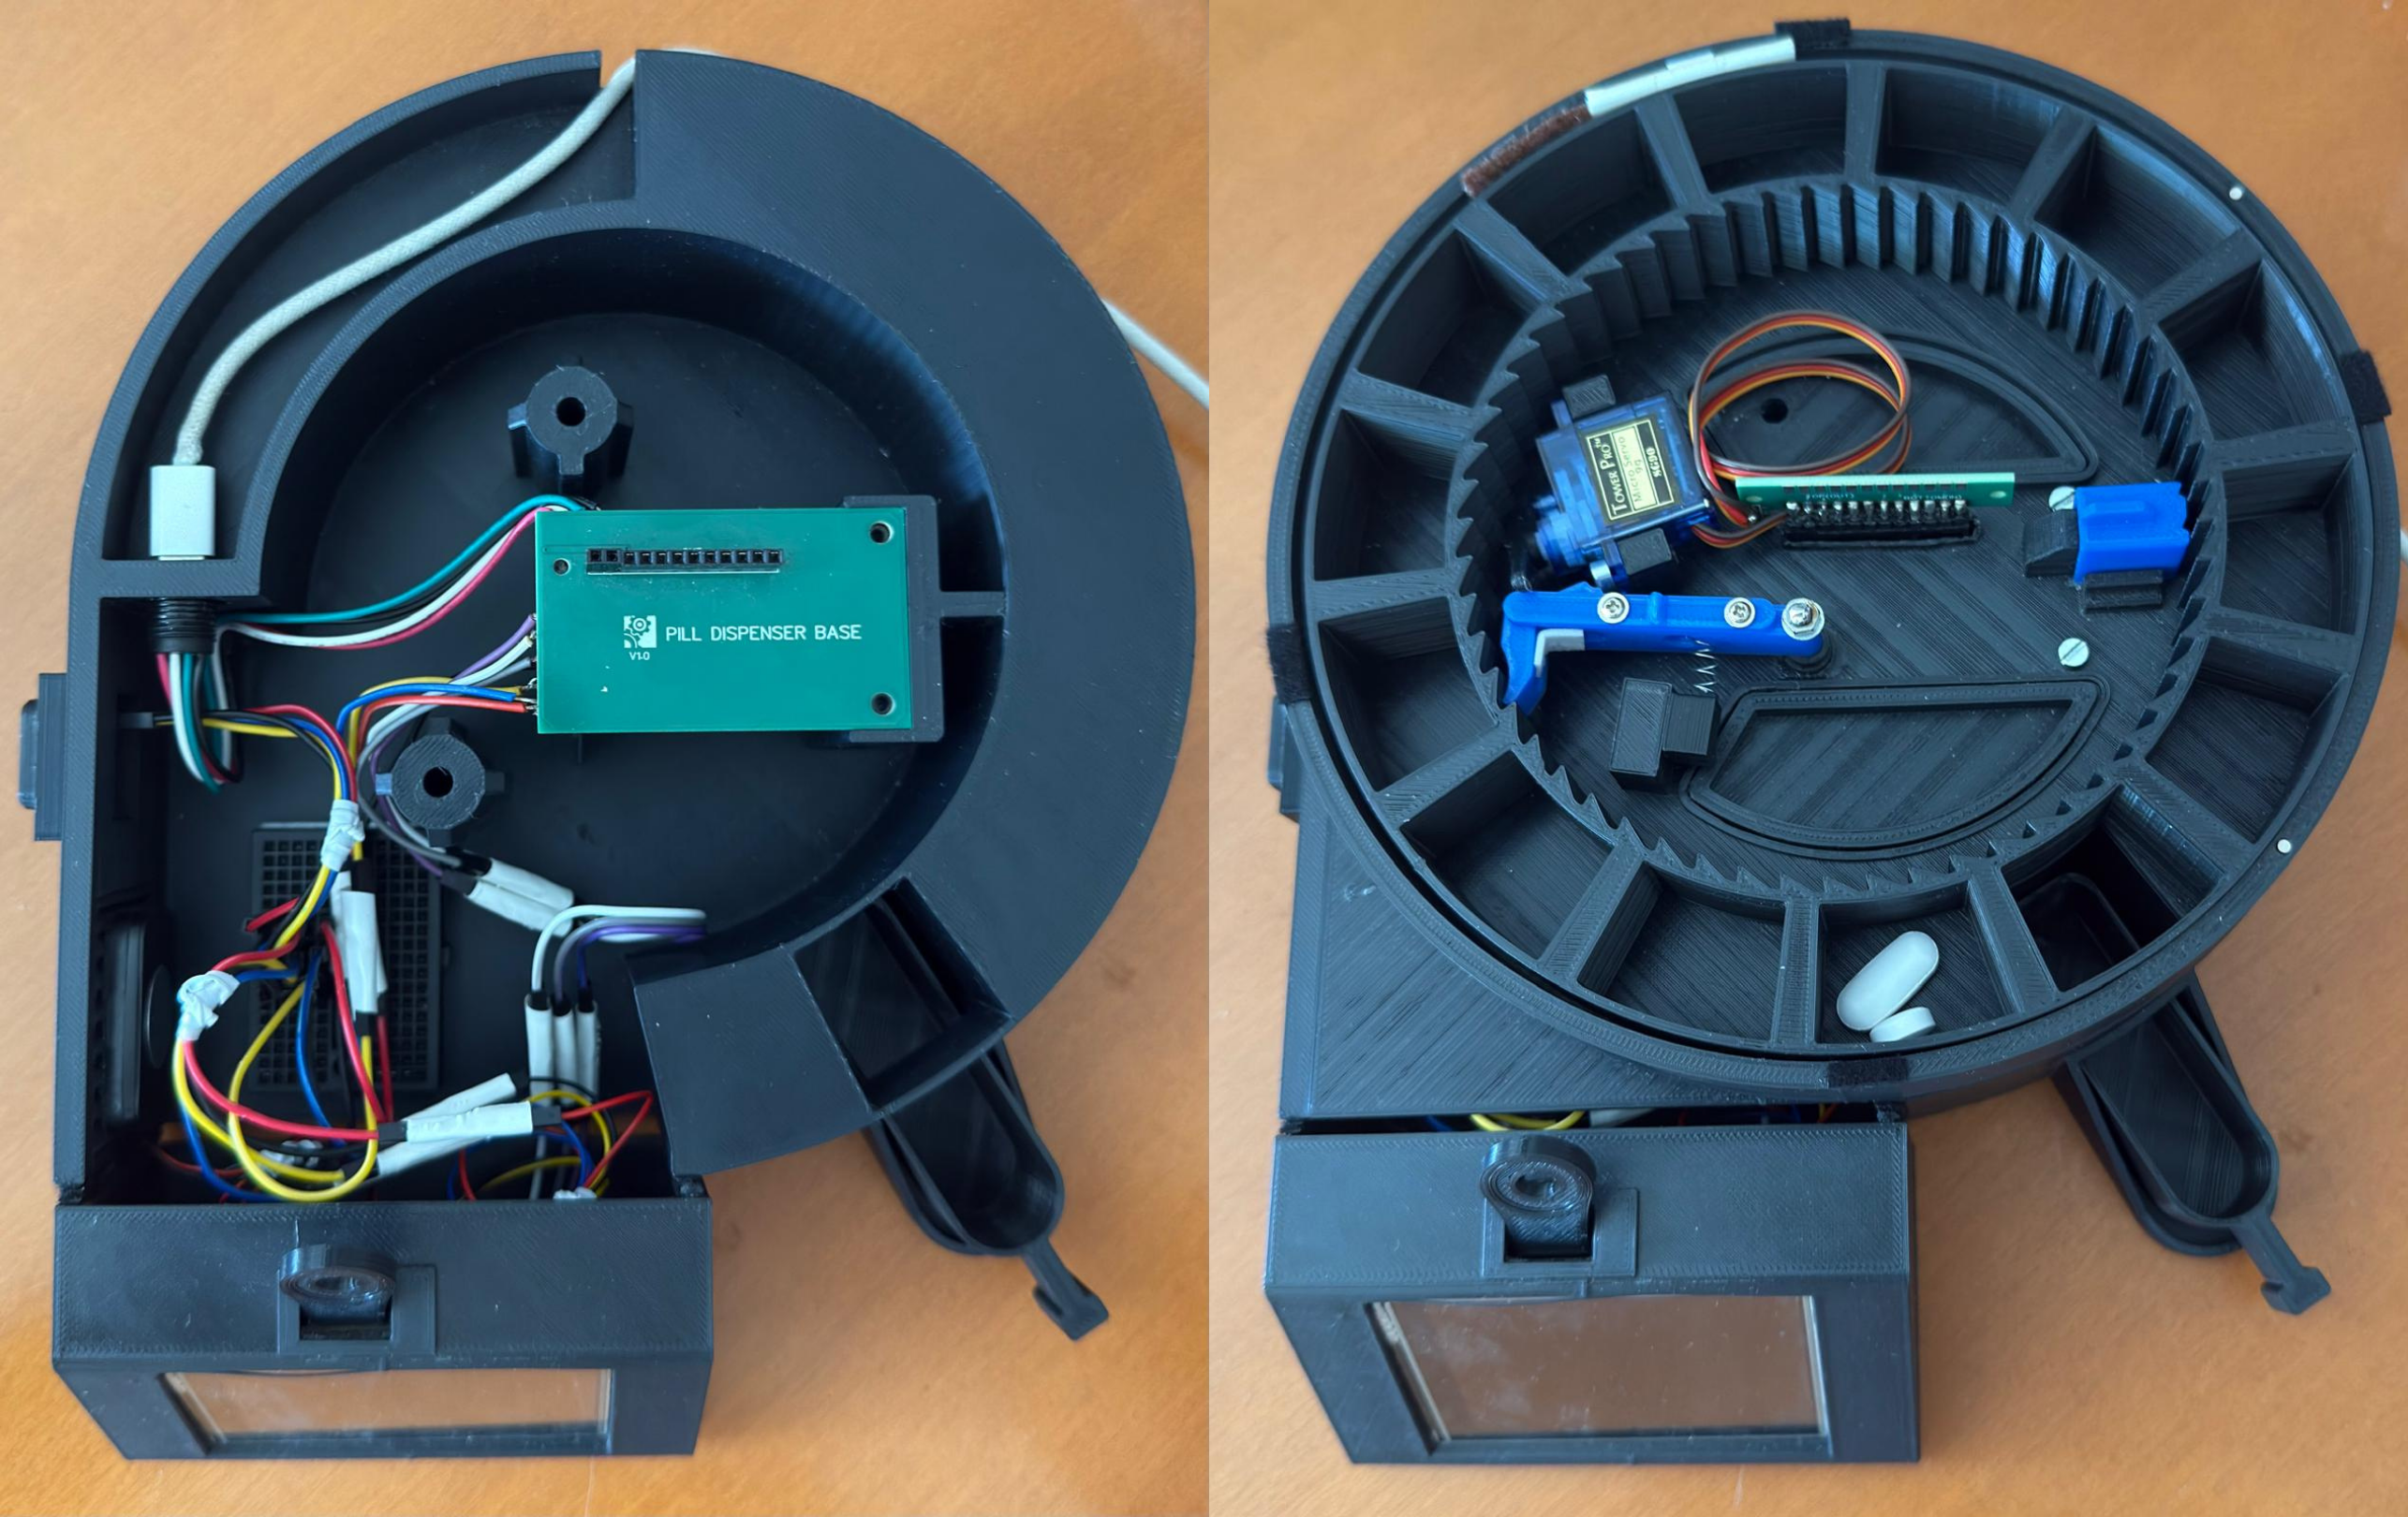
\includegraphics[width=0.5\textwidth]{figs/montaje.png}
    \caption{Integración hardware del sistema}
    \label{fig:montaje}
\end{figure}

\subsection{Relación hardware-software}
\label{sec:relacion_hw_sw}

El funcionamiento del sistema hardware está estrechamente ligado a la lógica de control implementada en el software.\\

En particular, el sistema de dispensación es activado en función de los eventos generados por la planificación de las tomas de medicamentos. Cuando se alcanza una hora programada, el sistema envía una señal de control al servomotor, provocando el movimiento del mecanismo de dispensación.\\

De forma similar, el sistema de sensado se activa bajo demanda desde la interfaz de usuario, permitiendo la adquisición de datos biomédicos en tiempo real.\\

Esta interacción entre hardware y software permite un funcionamiento coordinado del sistema, en el que cada componente físico actúa en respuesta a eventos gestionados por la lógica del dispositivo, garantizando un comportamiento predecible y fiable.
